\documentclass[9pt]{beamer}

% There are many different themes available for Beamer. A comprehensive
% list with examples is given here:
% http://deic.uab.es/~iblanes/beamer_gallery/index_by_theme.html

\usepackage[english]{babel}
\usepackage[TS1,T1]{fontenc}
\usepackage{array, booktabs}
\usepackage{multirow}
\usepackage[flushleft]{threeparttable}
\usepackage[font=small,labelfont=bf]{caption}
\usepackage[utf8]{inputenc}
\usepackage{bookman}
\usepackage{mathtools}
\usepackage{kotex}
\usepackage{adjustbox} % for \adjincludegraphics
\usepackage{textcomp}
\usepackage{pdfpages}

\newcommand\ytl[2]{\parbox[b]{8em}{\hfill{\color{cyan}\bfseries\sffamily #1}~$\cdot$~}\makebox[0pt][c]{$\bullet$}\vrule\quad \parbox[c]{4.5cm}{\vspace{7pt}\color{red!40!black!80}\raggedright\sffamily #2.\\[7pt]}\\[-3pt]}

\usefonttheme{professionalfonts}

\usetheme{metropolis}

\setbeamertemplate{caption}[numbered]{}
\setbeamertemplate{navigation symbols}{}
\setbeamertemplate{footline}[frame number]

%\setbeameroption{show notes}

\graphicspath{{images/}}

\title{\textbf{수치해석을 통한 지면에 고정된 캐비넷의 지진응답특성 분석}}

%\setbeamertemplate{footline}[text line]{%
%  \parbox{\linewidth}{\vspace*{-8pt}\small 2021년 한국지진공학회 학술발표대회\hfill\hfill\insertpagenumber}}
  
\setbeamertemplate{navigation symbols}{}

\subtitle{Numerical Analysis on Seismic Response of Cabinets Anchored to the Ground}

\author{김성용\inst{1}, 이철호\inst{2}, 전수찬\inst{3}, 배창준\inst{4}}
% - Give the names in the same order as the appear in the paper.
% - Use the \inst{?} command only if the authors have different
%   affiliation.

\institute[CWNU] % (optional, but mostly needed)
{
	\inst{1}%
	조교수, 창원대학교 건축공학과 | sungyong.kim@changwon.ac.kr\and
	\inst{2}%
	교수, 서울대학교 건축학과 \and
	\inst{2}%
	박사과정, 서울대학교 건축학과 \and
	\inst{2}%
	박사과정, 서울대학교 건축학과}
	
% - Use the \inst command only if there are several affiliations.
% - Keep it simple, no one is interested in your street address.

\date{2022/3/18 | 2021년도 한국지진공학회 학술발표대회}
% - Either use conference name or its abbreviation.
% - Not really informative to the audience, more for people (including
%   yourself) who are reading the slides online

\subject{Lecture Notes}
% This is only inserted into the PDF information catalog. Can be left
% out. 

% If you have a file called "university-logo-filename.xxx", where xxx
% is a graphic format that can be processed by latex or pdflatex,
% resp., then you can add a logo as follows:

% \pgfdeclareimage[height=0.5cm]{university-logo}{university-logo-filename}
% \logo{\pgfuseimage{university-logo}}


% Let's get started
\begin{document}

\begin{frame}
	\titlepage
\end{frame}

\section{Introduction}
	\begin{frame}
	\begin{figure}
	\centering
	\includegraphics[width=.89\textwidth]{image03}
	\caption{2016 경주지진과 2017 포항지진에 따른 비구조재 피해 사례}
	\label{fig:003}
\end{figure}

\begin{itemize}
	\item 2016 경주지진과 2017 포항지진으로 인해 커튼월, 유리 등 외장재 손상 및 낙하, 천장재 파손 및 낙하, 조적 비구조벽체, 치장벽체 균열 및 붕괴, 가스 및 수도 배관 파손 등 건축물 비구조요소 피해가 발생
	\item 지진시 비구조요소는 자체 손상, 낙하 및 전도로 직.간접적 인명 및 재산 피해뿐만 아니라 설비 및 중요 장비의 파손에 따른 건축물의 기능 상실로 2차 및 3차 피해로 연계되어 대규모 피해 발생 가능성이 높으므로 지진에 대한 안전성이 반드시 확보되어야 함
\end{itemize}
	\end{frame}
	\begin{frame}
	\begin{figure}[b!]
	\centering
	\includegraphics[scale=.40]{image01}
	\caption{건물에너지성능 관련 기준 동향}
	\label{fig:001}
\end{figure}
\begin{itemize}
	\item 최근 건설분야의 경우 제로에너지건축물에 대한 의무화 요구가 강력하게 추진되고 있음
	\item 2012년 연간에너지 소비량 당시 수준대비 5\%이던 에너지소비량을 2017년과 2025년에 이르기까지 30\%에서 60\%의 수준으로 낮추는 로드맵을 구축한 바 있다.
\end{itemize}
	\end{frame}
	\begin{frame}
\begin{figure}
\includegraphics[height=.95\textheight]{SINGLE_BASIC_DETAIL}
\caption{대상 열교차단 패스너 상세}
\end{figure}
	\end{frame}
	\begin{frame}
\begin{figure}
\includegraphics[height=.65\textheight]{SINGLE_BASIC_DRAWINGS_01}
\caption{대상 열교차단 패스너 설치도 및 분해도}
\end{figure}
	\end{frame}
	\begin{frame}
\begin{figure}
\includegraphics[height=.75\textheight]{image04}
\end{figure}
	\end{frame}
	\begin{frame}{연구개요}
	\textbf{GOAL:} (마감재 중량과 파스너 간격이 규정되지 않은 상황에서) 한계상태설계법에 따라 아래 하중조합에 의한 하중효과에 저항하도록 설계
	
	$\rightarrow$ 목표 설계가속도와 설계풍속에 대한 허용지지중량 및 파스너 간격 결정
	
	$\rightarrow$ 주어진 하중조건 하에서의 일종의 최적화 문제
	
	$\rightarrow$ 비구조재의 경우 건축구조물에 비해 단순한 시스템이기에 이러한 접근법이 가능 
	
\begin{itemize}
	\item[LC1] $1.4D$
	\item[LC2] $0.9D \pm 1.0E$
	\item[LC3] $0.9D \pm 1.3W$
\end{itemize}

%\begin{table}[h]
%\centering
%\caption{하중조합에 따른 소요압축강도 및 전단력}
%\label{tab:Demands}
%\begin{tabular}{@{}cccc@{}}
%\toprule
%하중조합 & 소요축력 $P_u$, kN & 수직방향 전단력 $V_v$, kN & 수평방향 전단력 $V_t$, kN \\ \midrule
%LC1  & 0 & 1.4$W_pg$ & 0 \\
%LC2  & 1.6$S_{DS}W_p$ & $(0.9g + 0.2S_{DS})W_p$ & 1.6$S_{DS}W_p$ \\
%LC3  & $1.3F_W$   & $0.9W_pg$                  & 0 \\ \bottomrule
%\end{tabular}
%\end{table}
%\vfill
	\end{frame}
\section{Governing Equation of Motion}
	\begin{frame}{Derivation}
	\begin{itemize}
		\item 만일 외장재의 타입과 상세가 미리 자세히 결정될 수 있다면, 건축물의 구조설계 과정이나 파스너 선정을 통한 외장재 부착방안을 개발할 때 외장재의 고정하중을 산정하고 그에 따른 구조적 검토 가능
		\item 구조설계 책임자가 프레임을 설계하고 외장재에 대한 부착 전략을 수립할 때 외장재는 일반적으로 결정/설계되지 않으며 건축물이나 파스너 업체의 구조설계 책임자가 외장재의 무게를 가정해야 함 
	\end{itemize}
\begin{figure}
\includegraphics[height=.40\textheight]{image05}
\end{figure}
	\end{frame}
	\begin{frame}{지진하중}
	지진하중 산정에 있어 본 검토에서는 고려할 수 있는 아래와 같은 가장 불리한 조건들을 가정함

\begin{itemize}
	\item 건물위치장소: 서울 지진구역(I), 지진구역계수(0.22g)
	\item 지반분류:  $S_5$ (보통암까지의 깊이 20m 이상)
	\item 내진등급: 1등급
	\item 비구조요소 설치위치: 건축물 최상층
\end{itemize}
	\end{frame}
	\begin{frame}{지진하중}
	비구조패널에 대한 등가정적 설계지진하중 $F_p$ (KDS 41 17 00:2019):

\begin{equation*}
	F_p = \frac{0.4a_pS_{DS}W_p}{R_p/I_p}\left(1+2\frac{z}{h}\right)
\end{equation*}

\noindent 여기서 설계지진하중 $F_p$는 다음의 값을 초과할 필요는 없으며, 

\begin{equation}
	F_p = 1.6S_{DS}I_pW_p
\end{equation}

\noindent $F_p$는 다음의 값 이상이 되어야 함: 

\begin{equation*}
	F_p = 0.3S_{DS}I_pW_p
\end{equation*}

\noindent 여기서 $a_p$는 1.0과 2.5 사이의 값을 갖는 증폭계수, $I_p$는 비구조요소의 중요도계수로서 1.0 또는 1.5, $h$는 구조물의 밑면으로부터 지붕층까지의 평균높이, $z$는 구조물의 밑면으로부터 비구조요소 위치까지의 높이, $R_p$는 비구조요소의 반응수정계수로서 1.0과 3.5 사이의 값, $S_{DS}$는 결정한 단주기에서의 설계스펙트럼가속도이고, $W_p$는 비구조요소의 가동중량.
	\end{frame}
	\begin{frame}{지진하중}
	수직방향 설계지진력 $F_{pv}$:

\begin{equation}
	F_{pv} = 0.2S_{DS}W_p.
\end{equation}

보수적인 판단을 위해 기타 연성의 비구조요소 중 변형에 제한된 부재 및 부착물에 대한 값으로 증폭계수는 2.5를, 반응수정계수는 접합시스테의 조임구에 대한 값인 1.0을 택하였으며, 이는 공진에 의한 응답의 증폭을 반영하되 후설치앵커를 통해 고정된다는 본 시스템의 특성 상 접합시스템의 연성이 구조물만큼 충분하지는 않다는 조건을 부여함

% Please add the following required packages to your document preamble:
% \usepackage{booktabs}
\begin{table}[]
\centering
\caption{건축비구조요소 또는 부재의 주요 계수값(KDS 41 17 00:2019)}
\label{tab:001}
\begin{tabular}{@{}ccc@{}}
\toprule
비구조요소        & 증폭계수 $a_p$    & 반응수정계수 $R_p$  \\ \midrule
변형이 제한된 기타 연성의 부재 및 부착물       & 2.5    & 2.5 \\
외측 비구조벽체 접합시스템의 조임구 & 1.25    & 1.0  \\ \bottomrule
\end{tabular}
\end{table}
	\end{frame}
	\begin{frame}{지진하중}
	\begin{figure}
\includegraphics[height=.40\textheight]{image06}
\end{figure}
	\end{frame}
	\begin{frame}{풍하중}
	본 검토에서는 다음의 조건을 고려함:  

\begin{itemize}
	\item 기본풍속 45m/s
	\item 노풍도 $C$
	\item 기준 높이 100m
	\item 밀폐형 건축물에 대한 기준 적용
	\item 경사가 없는 박공지붕에 대한 풍압계수 적용
\end{itemize}

외장재설계용 풍하중 $F_W$:

\begin{equation}
	F_W = p_C A_C
\end{equation}
 
\noindent 여기서 $p_C$는 외장재설계용 설계풍압 (N/m$^2$)이고, 단, 500 N/m$^2$ 보다 작아서는 안 되고, $A_C$는 외장재 등의 유효수압면적(m$^2$). 
	\end{frame}
	\begin{frame}{풍하중}
		\begin{figure}
\includegraphics[height=.40\textheight]{image07}
\end{figure}
	\end{frame}
	\begin{frame}{고려 하중조합}
	\begin{itemize}
	\item[LC1] $1.4D$
	\item[LC2] $0.9D + 1.0E$
	\item[LC3] $0.9D + 1.3W$
\end{itemize}

\begin{table}[h]
{\small\centering
\label{tab:Demands}
\begin{tabular}{@{}cccc@{}}
\toprule
하중조합 & 소요축력 $P_u$, kN & 수직방향 모멘트 $M_{ux}$, kN-m & 수평방향 모멘트 $M_{uy}$, kN-m \\ \midrule
LC1  & 0 & $1.4L_IW_pg$ & 0 \\
LC2  & $1.6S_{DS}W_p$ & $(0.9g + 0.2S_{DS})L_IW_p$ & $1.6S_{DS}L_IW_p$ \\
LC3  & $1.3p_CA_C$   & $0.9L_IW_pg$                  & 0 \\ \bottomrule
\end{tabular}}
\end{table}
	\end{frame}
	\begin{frame}{LC1에 대한 검토}
KDS 14 20 54:2016에 따르면 원형강봉에 대한 공칭휨강도 $M_n$은 항복강도(소성모멘트)로 다음과 같이 산정함:

\begin{equation*}
	M_n = M_p = F_{y,anc} Z_{anc} \leq 1.6M_y = 1.6F_{y,anc} S_{anc}
\end{equation*}

\noindent 여기서 $F_{y,anc}$는 앵커의 항복강도이고 $S_{anc}$와 $Z_{anc}$는 각각 탄성단면계수와 소성단면계수이며, 원형단면의 $Z_{anc}/S_{anc}=1.667$임에 따라 강봉의 휨강도는 최소값인 $1.6F_{y,anc}S_{anc}$로 산정됨.
  
중력하중에 대한 극한모멘트로부터 설계 만족조건은 아래와 같음: 

\begin{equation}
	1.4L_IW_pg \leq \phi_b 1.6F_{y,anc}S_{anc} \Rightarrow \frac{1.4L_IW_pg}{\phi_b 1.6F_{y,anc}S_{anc}} \leq 1.0 \Rightarrow f_{LC1}(W_pg) \leq 1.0
	\label{eq:fLC1}
\end{equation}

\noindent 여기서 $\phi_b$는 휨에 대한 강도저항계수(=0.90), $W_pg$는 앵커에 인가되는 중량이고, $L_I$는 단열재 두께(=강봉의 길이)임 
\end{frame}
\begin{frame}{LC2에 대한 검토}
KDS 14 20 54:2016에 따르면 2축 대칭단면 부재인 원형강봉에 있어서 휨과 압축력의 상관관계는 아래 식에 의해 제한됨 

\begin{subequations}
	\begin{equation*}
		\frac{P_u}{P_r}+\frac{8}{9}\left(\frac{M_{ux}^*}{M_{rx}}+\frac{M_{uy}^*}{M_{ry}}\right)\leq 1.0 ~~~ \textrm{for}~\frac{P_u}{P_r}\geq 0.2
	\end{equation*}
	\begin{equation*}
		\frac{P_u}{2P_r}+\left(\frac{M_{ux}^*}{M_{rx}}+\frac{M_{uy}^*}{M_{ry}}\right)\leq 1.0 ~~~ \textrm{for}~\frac{P_u}{P_r}< 0.2
	\end{equation*}
\end{subequations}

\noindent 여기서 $P_u$는 하중조합으로 구한 소요압축강도, $P_r$은 설계압축강도, $M_u^*$는 하중조합으로부터 압축력을 고려해 증폭된 모멘트를 반영한 소요증폭모멘트, $M_r$은 설계휨강도이고 $x, y$는 각각 강축과 약축 휨을 나타내는 아래첨자이며, 이를 단일 식으로 축약하면 아래와 같음:

\begin{equation}
	\frac{1}{C_1}\left(\frac{M_{ux}^*}{M_{rx}} + \frac{M_{uy}^*}{M_{rx}}\right) + \frac{P_u}{C_2P_r} \leq 1.0 \Rightarrow f_{LC2}(W_pg;S_{DS}) \leq 1.0
	\label{eq:fLC2}
\end{equation}

\noindent 여기서 $C_1$과 $C_2$는 각각 $P_u/P_r<0.2$일 때는 9/8와 1이고, 그 외에는 1과 2.

\end{frame}
\begin{frame}{LC3에 대한 검토}

KDS 14 20 54:2016에 따르면 2축 대칭단면 부재인 원형강봉에 있어서 휨과 압축력의 상관관계는 아래 식에 의해 제한됨 

\begin{subequations}
	\begin{equation*}
		\frac{P_u}{P_r}+\frac{8}{9}\frac{M_{ux}^*}{M_{rx}}\leq 1.0 ~~~ \textrm{for}~\frac{P_u}{P_r}\geq 0.2
	\end{equation*}
	\begin{equation*}
		\frac{P_u}{2P_r}+\frac{M_{ux}^*}{M_{rx}}\leq 1.0 ~~~ \textrm{for}~\frac{P_u}{P_r}< 0.2
	\end{equation*}
\end{subequations}

\noindent 여기서 $P_u$는 하중조합으로 구한 소요압축강도, $P_r$은 설계압축강도, $M_u^*$는 하중조합으로부터 압축력을 고려해 증폭된 모멘트를 반영한 소요증폭모멘트, $M_r$은 설계휨강도이고 $x, y$는 각각 강축과 약축 휨을 나타내는 아래첨자이며, 이를 단일 식으로 축약하면 아래와 같음:

\begin{equation}
	\frac{1}{C_1}\frac{M_{ux}^*}{M_{rx}} + \frac{P_u}{C_2P_r} \leq 1.0 \Rightarrow f_{LC3}(W_pg, A_C;S_{DS}, p_C) \leq 1.0
	\label{eq:fLC3}
\end{equation}

\noindent 여기서 $C_1$과 $C_2$는 각각 $P_u/P_r<0.2$일 때는 9/8와 1이고, 그 외에는 1과 2.
\end{frame}
	\begin{frame}{Problem Formulation}
	Find the optimal tradeoff between $W_pg$ and $A_C$:
	
	subject to $g(W_pg,A_C;S_{DS},p_C)=\max(f_{LC1},f_{LC2},f_{LC3})\leq 1.0$
	
	\noindent where $f_{LC1}=f_{LC1}(W_pg)$, $f_{LC2}=f_{LC2}(W_pg;S_{DS})$, and $f_{LC3}=f_{LC3}(W_pg, A_C;S_{DS}, p_C)$ are defined as Eqs. \eqref{eq:fLC1}, \eqref{eq:fLC2}, and \eqref{eq:fLC3}, respectively. 
	\end{frame}	
	\begin{frame}{Design Results}
		\begin{figure}
\includegraphics[height=.40\textheight]{Result01}
\includegraphics[height=.40\textheight]{Result02}
\caption{$S_{DS}=0.4766\mathrm g$, $p_C=5380\mathrm N$ (left), and $S_{DS}=0.2766\mathrm g$, $p_C=5380\mathrm N$ (right)}
\end{figure}	
	\end{frame}
	\begin{frame}{Design Results}
		\begin{figure}
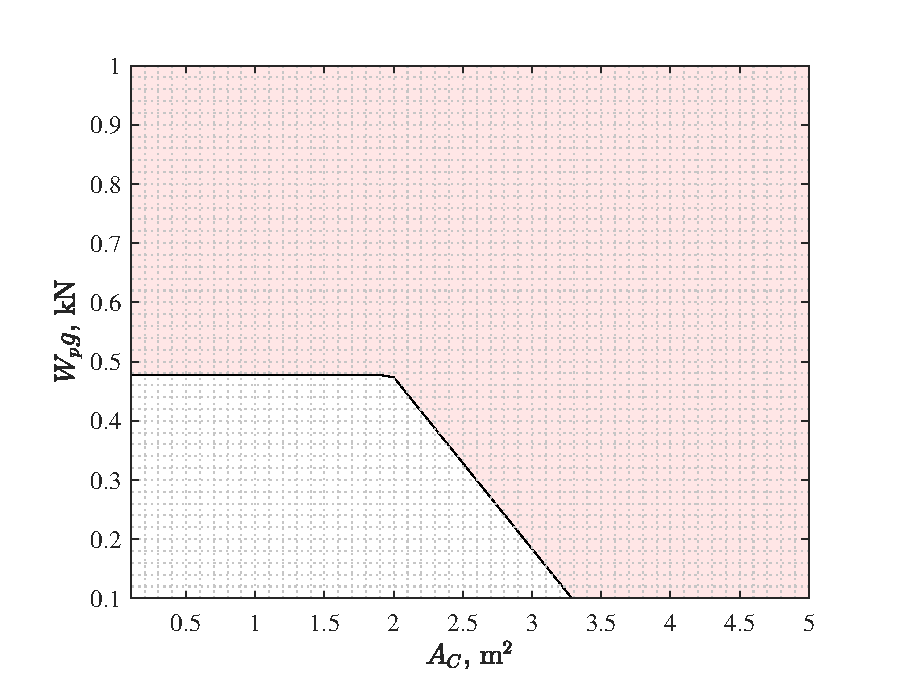
\includegraphics[height=.40\textheight]{Result03}
\includegraphics[height=.40\textheight]{Result04}
\caption{$S_{DS}=0.4766\mathrm g$, $p_C=8230\mathrm N$ (left), and $S_{DS}=0.2766\mathrm g$, $p_C=8230\mathrm N$ (right)}
\end{figure}	
	\end{frame}
	\begin{frame}{Conclusions and Future Works}
\begin{itemize}
	\item 내풍과 내진성능을 고려한 파스너의 허용지지중량 및 파스너가 개당 받을 수 있는 면적을 산정함
	\item 마감재 중량과 파스너 간격이 규정되지 않은 상황에서의 주어진 하중조건에 대한 일반적 해가 도출됨
	\item 단순한 형태의 비선형방정식을 토대로 설계치가 결정되었는데, 이는 복잡한 건축물 대비 단순한 메커니즘을 통해 하중을 전달하는 비구조재의 특성에 기인함
	\item 차후 동일한 논리를 동적거동에 대한 경우로 확장할 예정이며, 간편하게 허용중량 및 허용간격을 얻을 수 있는 도표나 그림 도출 예정
\end{itemize}
	\end{frame}
	\begin{frame}
		경청해 주셔서 감사합니다. 
	\end{frame}
\end{document}
